\documentclass[tikz,convert={outfile=\jobname.svg}]{standalone}
\usepackage{amsmath}
\usepackage{pgfplots}
\begin{document}
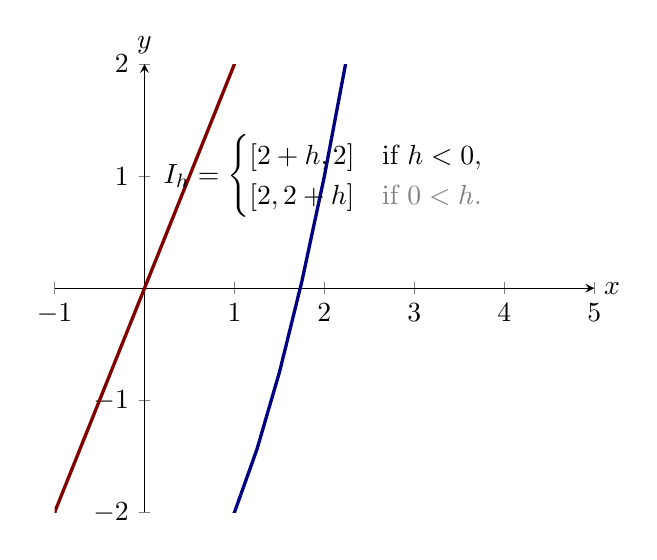
\begin{tikzpicture}
  \colorlet{background}{white}
  \colorlet{textColor}{black}
  \colorlet{penColor}{blue!50!black}
  \colorlet{penColor2}{red!50!black}
	\begin{axis}[
            domain=-1:5,
            xmax=5,
            xmin=-1,
            ymax=2,
            ymin=-2,
            axis lines =middle, xlabel=$x$, ylabel=$y$,
            every axis y label/.style={at=(current axis.above origin),anchor=south},
            every axis x label/.style={at=(current axis.right of origin),anchor=west}
          ]
          \addplot [very thick, penColor] {x^2-3};
          \addplot [very thick, penColor2] {2*x};
          \node at (axis cs:2,1) {$I_h = \begin{cases}[2+h,2]  & \text{if $h<0$}, \\ [2,2+h]  & \color{gray}\text{if $0<h$}.\end{cases}$};  
          \node at (axis cs:.8,3) {\color{penColor2}$f'(x)$};
        \end{axis}
\end{tikzpicture}
\end{tikzpicture}
\end{document}
